 % The main file for CAMP reports
 % Don't put any content in here. 
 % Don't even include content files by using \input or \inlcude. 
 % Put your content to TEXT.TEX or include it there using \input.
 % Uses:
 %		SETTINGS.TEX	contains the settings for this document
 %		COMMANDS.TEX	contains commands which can be used while writing
 %		INFO.TEX			contains the author, title and so on for the cover
 %		COVER.TEX			formats the front cover of the document
 %		ABSTRACT.TEX	contains the abstract to be included (if needed)
 %		TEXT.TEX			contains the actual content of the document
 %		BIB.BIB				containt the BibTeX entries for the document
 
 
%% Draft document mode
%% Final document
\documentclass[11pt,a4paper,bibtotoc,idxtotoc,headsepline,footsepline,footexclude,BCOR12mm,DIV13]{scrbook}

%\documentclass[11pt,a4paper,bibtotoc,idxtotoc,headsepline,footsepline,footexclude,BCOR20mm,DIV10]{scrbook}

% KOMA-Optionen:
%  bibtotoc: include bibliography in table of contents
%  idxtotoc: include index in table of contents
%  headsepline: use horizontalline under heading
%  BCOR: binding correcion (Bindungskorrektur) (e.g.: BCOR5mm)
%  DIV: Number of sheet sections (used for layout) (e.g.: DIV12) 



% include title and author information for the cover
% Set here the title, authors and other stuff to be used for the cover
% This file is used by MAIN.TEX

% set title, authors and stuff for the cover
\def\doctype{Projekt in Datenbanksysteme}
\def\title{Wahlinformationssystem f�r die Bundestagswahl}
\def\author{Korbinian Schmid und Pascal Minnerup}
\def\date{Januar 05, 2011}

% text to appear in the footer
\def\footertext{}

% include settings
% Included by MAIN.TEX
% Defines the settings for the CAMP report document

\renewcommand{\sectfont}{\normalfont \bfseries}        % Schriftart der Kopfzeile

% manipulate footer
\usepackage{scrpage2}
\pagestyle{scrheadings}
\ifoot[\footertext]{\footertext} % \footertext set in INFO.TEX
%\setkomafont{pagehead}{\normalfont\rmfamily}
\setkomafont{pagenumber}{\normalfont\rmfamily}

%% allow sophisticated control structures
\usepackage{ifthen}

% use Palatino as default font
\usepackage{palatino}

% enable special PostScript fonts
\usepackage{pifont}

% make thumbnails
\usepackage{thumbpdf}

%to use the subfigures
\usepackage{subfigure}


\usepackage{colortbl}


%% show program code\ldots
%\usepackage{verbatim}
%\usepackage{program}

%% enable TUM symbols on title page
\usepackage{styles/tumlogo}


% Use listing environment for SQL code
\usepackage{listings}


\usepackage{multirow}

%% use colors
\usepackage{color}

%% make fancy math
\usepackage{amsmath}
\usepackage{amsfonts}
\usepackage{amssymb}
\usepackage{textcomp}
\usepackage{yhmath} % f�r die adots 
%% mark text as preliminary
%\usepackage[draft,german,scrtime]{prelim2e}

%% create an index
\usepackage{makeidx}

% for the program environment
\usepackage{float}

%% load german babel package for german abstract
%\usepackage[german,american]{babel}
\usepackage[german,english]{babel}
\selectlanguage{english}

% use german characters as well
\usepackage[latin1]{inputenc}       % allow Latin1 characters

% use initals dropped caps - doesn't work with PDF
%\usepackage{dropping}


\usepackage{styles/shortoverview}
%----------------------------------------------------
%      Graphics and Hyperlinks
%----------------------------------------------------

%% check for pdfTeX
\ifx\pdftexversion\undefined
 %% use PostScript graphics
 \usepackage[dvips]{graphicx}
 \DeclareGraphicsExtensions{.eps,.epsi}
 \graphicspath{{figures/}{figures/review}} 
 %% allow rotations
 \usepackage{rotating}
 %% mark pages as draft copies
 %\usepackage[english,all,light]{draftcopy}
 %% use hypertex version of hyperref
 \usepackage[hypertex,hyperindex=false,colorlinks=false]{hyperref}
\else %% reduce output size \pdfcompresslevel=9
 %% declare pdfinfo
 %\pdfinfo { 
 %  /Title (my title) 
 %  /Creator (pdfLaTeX) 
 %  /Author (my name) 
 %  /Subject (my subject	) 
 %  /Keywords (my keywords)
 %}
 %% use pdf or jpg graphics
 \usepackage[pdftex]{graphicx}
 \DeclareGraphicsExtensions{.jpg,.JPG,.png,.pdf,.eps}
 \graphicspath{{figures/}} 
 
 %% Load float package, for enabling floating extensions
 \usepackage{float}
 
 %% allow rotations
 \usepackage{rotating}
 %% use pdftex version of hyperref
 \usepackage[pdftex,colorlinks=true,linkcolor=red,citecolor=red,%
 anchorcolor=red,urlcolor=red,bookmarks=true,%
 bookmarksopen=true,bookmarksopenlevel=0,plainpages=false%
 bookmarksnumbered=true,hyperindex=false,pdfstartview=%
 ]{hyperref}
%
%\usepackage[pdftex,colorlinks=false,linkcolor=red,citecolor=red,%
% anchorcolor=red,urlcolor=red,bookmarks=true,%
% bookmarksopen=true,bookmarksopenlevel=0,plainpages=false%
% bookmarksnumbered=true,hyperindex=false,pdfstartview=%
% ]{hyperref}
\fi




%% Fancy chapters
%\usepackage[Lenny]{fncychap}
%\usepackage[Glenn]{fncychap}
%\usepackage[Bjarne]{fncychap}

%\usepackage[avantgarde]{quotchap}

% set the bibliography style
%\bibliographystyle{styles/bauermaNum}
%\bibliographystyle{alpha}
\bibliographystyle{plain}

% include commands
% Commands to be used within the TUM report document
% Included by MAIN.TEX
% Please include your own cool commands here. 
% Be only sure to comment it sufficiently so others can use it.

%-------------------------------------------------------------
%                      Own Commands
%-------------------------------------------------------------


%-------------------------------------------------------------
% math stuff -------------------------------------------------

% nice R, N, C
\newcommand{\nat}{\mathbb{N}}
\newcommand{\real}{\mathbb{R}}
\newcommand{\compl}{\mathbb{C}}



% norm
\newcommand{\norm}[1]{\left\| #1 \right\|}

% un demi
\newcommand{\half}{\frac{1}{2}}

% parantheses
\newcommand{\parenth}[1]{ \left( #1 \right) }
\newcommand{\bracket}[1]{ \left[ #1 \right] }
\newcommand{\accolade}[1]{ \left\{ #1 \right\} }
%\newcommand{\angle}[1]{ \left\langle  #1 \right\rangle }

% partial derivative: %#1 function, #2 which variable
% simple / single line version
\newcommand{\pardevS}[2]{ \delta_{#1} f(#2) }
% fraction version
\newcommand{\pardevF}[2]{ \frac{\partial #1}{\partial #2} }

% render vectors: 3 and 4 dimensional
\newcommand{\veciii}[3]{\left[ \begin{array}[h]{c} #1 \\ #2 \\ #3	\end{array} \right]}
\newcommand{\veciv}[4]{\left[ \begin{array}[h]{c} #1 \\ #2 \\ #3 \\ #4	\end{array} \right]}

% render matrices: 3  dimensional (arguments in row first order)
\newcommand{\matiii}[9]{\left[ \begin{array}[h]{ccc} #1 & #2 & #3 \\ #4 & #5 & #6 \\ #7 & #8 & #9	\end{array} \right]}
%DOESN'T WORK,DON'T KNOW WHY \newcommand{\mativ}[16]{\left[ \begin{array}[h]{cccc} #1 & #2 & #3 & #4 \\ #5 & #6 & #7 & #8 \\ #9 & #10 & #11 & #12 \\ #13 & #14 & #15 & #16 \end{array} \right]}


%-------------------------------------------------------------
%-------------------------------------------------------------


%-------------------------------------------------------------
% some abreviations ------------------------------------------
\newcommand{\Reg}{$^{\textregistered}$}
\newcommand{\reg}{$^{\textregistered}$ }
\newcommand{\Tm}{\texttrademark}
\newcommand{\tm}{\texttrademark~}
\newcommand {\bsl} {$\backslash$}

%-------------------------------------------------------------
%-------------------------------------------------------------


%-------------------------------------------------------------
% formating --------------------------------------------------

% Theorem & Co environments and counters
\newtheorem{theorem}{Theorem}[chapter]
\newtheorem{lemma}[theorem]{Lemma}
\newtheorem{corollary}[theorem]{Corollary}
\newtheorem{remark}[theorem]{Remark}
\newtheorem{definition}[theorem]{Definition}
\newtheorem{equat}[theorem]{Equation}
\newtheorem{example}[theorem]{Example}
\newtheorem{algorithm}[theorem]{Algorithm}

% inserting figures
\newcommand{\insertfigure}[4]{ % Filename, Caption, Label, Width percent of textwidth
	\begin{figure}[htbp]
		\begin{center}
			\includegraphics[width=#4\textwidth]{#1}
		\end{center}
		\vspace{-0.4cm}
		\caption{#2}
		\label{#3}
	\end{figure}
}




% referecing figures

\newcommand{\refFigure}[1]{ %label
	figure \ref{#1}
}
\newcommand{\refChapter}[1]{ %label
	chapter \ref{#1}
}

\newcommand{\refSection}[1]{ %label
	section \ref{#1}
}

\newcommand{\refParagraph}[1]{ %label
	paragraph \ref{#1}
}

\newcommand{\refEquation}[1]{ %label
	equation \ref{#1}
}

\newcommand{\refTable}[1]{ %label
	table \ref{#1}
}




\newcommand{\rigidTransform}[2]
{
	${}^{#2}\!\mathbf{H}_{#1}$
}

%code, in typewriter
\newcommand{\code}[1]
 {\texttt{#1}}

% comment that appears on the border - very practical !!!
\newcommand{\comment}[1]{\marginpar{\raggedright \noindent \footnotesize {\sl #1} }}

% page clearing
\newcommand{\clearemptydoublepage}{%
  \ifthenelse{\boolean{@twoside}}{\newpage{\pagestyle{empty}\cleardoublepage}}%
  {\clearpage}}


%-------------------------------------------------------------
%-------------------------------------------------------------


\newcommand{\etAl}{\emph{et al.}\mbox{ }}


%\makeindex
	%% inter line spacing
%\linespread{1.0}

\makeglossary

\begin{document}

	\frontmatter
	
	
	% The front cover for the TUM report document.
% Included by MAIN.TEX


%--------------------------------------------------
% The Front Cover
%--------------------------------------------------

% The front cover for the TUM document.
% Included by MAIN.TEX


%--------------------------------------------------
% The Front Cover
%--------------------------------------------------

% correct BCOR - undo at the end !!!
\def\bcorcor{0.15cm}
\addtolength{\hoffset}{\bcorcor}

\thispagestyle{empty}

 \vspace{4cm}
\begin{center}
	       \oTUM{4cm}
	   
	   \vspace{5mm}     
	   \huge FAKULT{\"A}T F{\"U}R INFORMATIK\\ 
	   \vspace{0.5cm}
	 \large DER TECHNISCHEN UNIVERSIT{\"A}T M{\"U}NCHEN\\
    \vspace{1mm}
        
	\end{center}
		

\vspace{15mm}
\begin{center}

   {\Large \doctype}

  \vspace{20mm}
  
  {\huge\bf \title}\\%[3ex]
  
  
  \vspace{15mm}
  
  
  {\LARGE  \author}
  
  \vspace{10mm}
  
  \begin{figure}[h!]
  \centering
   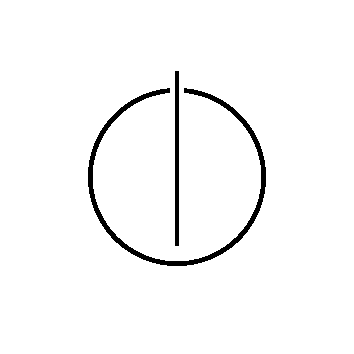
\includegraphics[width=4cm]{styles/informat.png}
  \end{figure}
  
  \end{center}
%	\clearemptydoublepage
	
	
	% Abstract for the TUM report document
% Included by MAIN.TEX


\clearemptydoublepage
\phantomsection
\addcontentsline{toc}{chapter}{Abstract}	





\vspace*{2cm}
\begin{center}
{\Large \bf Abstract}
\end{center}
\vspace{1cm}

Im Rahmen der Vorlesung Datenbanksysteme erstellen die Studenten ein Wahlinformationsystem f�r die Bundestagswahl. Das Wahlinformationssystem umfasst die Generierung der Ausgangsdaten, das aggregieren und auswerten dieser Daten, sowie die Pr�sentation auf einer Webseite. Au�erdem enth�lt es ein Benchmarksystem um die Performanz zu testen.

	\tableofcontents

	\mainmatter
	
			\chapter{Modellierung des Wahlinformationssystems}

Hier wird das ER Modell usw. vorgestellt.
 



		
			\section{Informationsstrukturanforderungen}

Die L�ngenangaben sind jeweils in Byte.


\newcommand{\StartTabelle}[2]{
	\textbf{Objektbeschreibung:} #1
	\begin{itemize}
		\item Anzahl: #2
		\item Attribute:
			\begin{itemize}
}

\newcommand{\DefAttribut}[7]{
	\item Attributname: #1
		\begin{itemize}
			\item L�nge: #2
			\item Wertebereich: #3
			\item Wiederholungen: #4
			\item Definiertheit: #5
			\item Identifizierend: #6
		\end{itemize}
}

\newcommand{\EndeTabelle}{
	\end{itemize}
	\end{itemize}
}


%Objektbeschreibung: T1
%\begin{itemize}
%	\item Anzahl: T2
%	\item Attribute:
%		\begin{itemize}
%			\item Attributname: T3
%			\begin{itemize}
%				\item L�nge: T4
%				\item Wertebereich: T5
%				\item Wiederholungen: T6
%				\item Definiertheit: T7
%				\item Identifizierend: T8
%			\end{itemize}
%		\end{itemize}
%\end{itemize}
%
%\newcommand{\StartTabelle}[2]{
%	\begin{table}[htbp]
%		\centering
%			\begin{tabular}{llllllll}
%		\textbf{Objektbeschreibung:} & #1\\
%		\textbf{Anzahl:} & #2\\
%		\textbf{Attribute:} \\
%		\textbf{Attributname} & \textbf{type} & \textbf{L�nge} & \textbf{Wertebereich} & \textbf{\#Wdh.} & \textbf{Def'heit} & \textbf{Id.} \\
%}
%
%\newcommand{\DefAttribut}[7]{#1 & #2 & #3 & #4 & #5 & #6 & #7 \\}
%
%\newcommand{\EndeTabelle}{
%	\end{tabular}
%	\end{table}
%}

\newcommand{\DefIDTabelle}[2]{
	\StartTabelle{#1}{#2}
		\DefAttribut{ID}{int}{4}{0 ... #2}{0}{100\%}{ja}
	\EndeTabelle
}

\newcommand{\DefShortString}[1]{\DefAttribut{#1}{char}{50}{*}{0}{100\%}{nein}}
\newcommand{\DefString}[2]{\DefAttribut{#1}{char}{#2}{*}{0}{100\%}{nein}}
\newcommand{\DefID}[1]{\DefAttribut{ID}{int}{4}{0 ... #1}{0}{100\%}{ja}}

\DefIDTabelle{Wahlbezirk}{25.000}

\StartTabelle{Wahlkreis}{299}
	\DefID{299}
	\DefShortString{Wahlkreisname}
\EndeTabelle

\StartTabelle{Bundesland}{16}
	\DefID{16}
	\DefShortString{Name}
\EndeTabelle

\StartTabelle{Kandidat}{5000}
	\DefID{5000}
	\DefShortString{Name}
	\DefShortString{Vorname}
	\DefString{Beruf}{255}
	\DefString{Anschrift}{2047}
	\DefAttribut{Geburtsdatum}{date}{4}{*}{0}{100\%}{ja}
	\DefShortString{Geburtsort}
\EndeTabelle

\StartTabelle{Partei}{50}
	\DefID{50}
	\DefShortString{Name}
	\DefShortString{K�rzel}
\EndeTabelle

\StartTabelle{Stimme}{50.000.000}
	\DefID{50.000.000}
	\DefAttribut{Jahr}{int}{4}{1900 ... 2100}{0}{100\%}{nein}
\EndeTabelle

\StartTabelle{Wahlberechtigter}{50.000.000}
	\DefID{50.000.000}
	\DefAttribut{Gew�hlt}{int}{1}{0, 1}{0}{50\%}{nein}
\EndeTabelle

\StartTabelle{ErstStimmenNachWahlkreis}{10.000}
	\DefAttribut{Anzahl}{int}{4}{0 ... 200.000}{0}{100\%}{nein}
	\DefAttribut{Jahr}{int}{4}{1900 ... 2100}{0}{100\%}{nein}
\EndeTabelle

\StartTabelle{ZweitStimmenNachWahlkreis}{10.000}
	\DefAttribut{Anzahl}{int}{4}{0 ... 200.000}{0}{100\%}{nein}
	\DefAttribut{Jahr}{int}{4}{1900 ... 2100}{0}{100\%}{nein}
\EndeTabelle

\StartTabelle{WahlkreisDaten}{10.000}
	\DefID{10.000}
	\DefAttribut{AnzahlWahlberechtigte}{int}{4}{0 ... 200.000}{0}{100\%}{nein}
	\DefAttribut{AnzahlUngueltigeErststimmen}{int}{4}{0 ... 200.000}{0}{100\%}{nein}
	\DefAttribut{AnzahlUngueltigeZweitstimmen}{int}{4}{0 ... 200.000}{0}{100\%}{nein}
	\DefAttribut{Jahr}{int}{4}{1900 ... 2100}{0}{100\%}{nein}
\EndeTabelle

Beziehungsbeschreibung: w�hlt (1. Stimme)\\
- Beteiligte Objekte:\\
    Stimme als W�hler\\
    Kandidat als Empf�nger der Stimme\\
- Anzahl: 45.000.000\\

Beziehungsbeschreibung: w�hlt (2. Stimme)\\
- Beteiligte Objekte:\\
    Stimme als W�hler\\
    Partei als Empf�nger der Stimme\\
- Anzahl: 45.000.000\\
			
			\section{Datenverarbeitungsanforderungen}

Das Wahlsystem soll unter anderem die folgenden Datenverarbeitungsoperationen unterst�tzen. Die nachfolgenden Daten sind Sch�tzungen, die vor der Implementierun erhoben wurden.

\textbf{Prozessbeschreibung:} Berechnung Wahlbeteiligung
\begin{itemize}
	\item H�ufigkeit: j�hrlich
	\item ben�tigte Daten:
		\begin{itemize}
			\item Stimmen
    	\item Wahlbezirke
    	\item Wahlkreise
    	\item Bundesl�nder
		\end{itemize}
	\item Priorit�t: hoch
	\item zu verarbeitende Menge
		\begin{itemize}
			\item 45.000.000 Stimmen
			\item 2500 Wahlbezirke
			\item 299 Wahlkreise
			\item 16 Bundesl�nder
		\end{itemize}  
\end{itemize}

\textbf{Prozessbeschreibung}: Berechnung Wahlergebnis
\begin{itemize}
	\item H�ufigkeit: j�hrlich
	\item ben�tigte Daten:
		\begin{itemize}
			\item Stimmen
			\item Parteien
			\item Kandidaten
			\item Wahlbezirke
			\item Wahlkreise
			\item Landeslisten
		\end{itemize}
	\item Priorit�t: hoch
	\item zu verarbeitende Menge
		\begin{itemize}
			\item 45.000.000 Stimmen
    	\item 30 Parteien
			\item 2.500 Kandidaten
			\item 2.500 Wahlbezirke
			\item 299 Wahlkreise
			\item 500 Landeslisten
		\end{itemize}
\end{itemize}

\textbf{Prozessbeschreibung}: Berechnung Sitzverteilung
\begin{itemize}
	\item H�ufigkeit: j�hrlich
	\item ben�tigte Daten:
		\begin{itemize}
			\item Stimmen
    	\item Parteien
    	\item Kandidaten
    	\item Wahlbezirke
    	\item Wahlkreise
    	\item Landeslisten
    \end{itemize}
	\item Priorit�t: hoch
	\item zu verarbeitende Menge
		\begin{itemize}
			\item 50.000.000 Stimmen
    	\item 30 Parteien
    	\item 2.500 Kandidaten
    	\item 2.500 Wahlbezirke
    	\item 299 Wahlkreise
    	\item 500 Landeslisten
		\end{itemize}
\end{itemize}

			
			\chapter{Vor- und Nachteile Eines DBMS}

\textbf{Vorteile:}
\begin{itemize}
    \item Verhindern von Redundanz und Inkonsistenz
    \item Einheitliche Modellierung der Informationen und damit erweiterte Zugriffsm�glichkeiten
    \item M�glichkeit des Mehrbenutzerbetriebes
    \item Vorbeugung gegen Datenverlust
    \item Durchsetzung von Integrit�tsbedingungen
    \item Durchsetzung von Sicherheitsmechanismen
    \item Niedrigere Entwicklungskosten f�r neue Anwendungsprogramme
\end{itemize}



\textbf{Nachteile:}
\begin{itemize}
    \item Kosten f�r Anschaffung und Betrieb des DBMS
    \item Gegen�ber Papierl�sungen: Angreifbarkeit durch Computerviren
    \item M�gliche Abh�ngigkeit von einer einzelnen Software
\end{itemize}
			
			\section{Integrit�tsbedingungen}
\begin{itemize}
    \item Jeder Listenplatz darf maximal einmal vergeben werden.
    \item Die Funktionalit�ten m�ssen eingehalten werden
    \item Eine Erststimme kann nur einem Kandidaten gegeben werden, der in dem Wahlkreis des Wahlbezirkes der Stimme f�r ein Direktmandat kandidiert.
    \item Eine Zweitstimme kann nur einer Partei gegeben werden, die eine Landesliste in dem Bundesland hat, in dem der Wahlkreis des Wahlbezirkes der Stimme liegt.
    \item Jede Partei darf in jedem Bundesland maximal eine Landesliste haben.
    \item Ein Kanditat, der Mitglied einer Partei ist, darf nicht f�r eine andere Partei kandidieren.
\end{itemize}
			
			\section{Datenschutzanforderungen}

Um den Datenschutz zu gew�hrleisten wird als ersten Schritt nach Vorlage des Personalausweises ein W�hlpasswort generiert, mit dem der Wahlberechtigte abstimmen kann. Ab dem Zeitpunkt ist seine Stimme entkoppelt von seinem Personalausweis und somit sind R�ckschl�sse nicht mehr direkt m�glich. Indirekte R�ckschl�sse werden dadurch erschwert, dass die Auswertung erst nach Schlie�ung der Wahllokale erfolgt und somit immer gro�e Stimmzettel-Mengen aggregiert werden. Insbesondere ist es dadurch nicht m�glich die Wahlkreisergebnisse direkt vor der Stimmabgabe einer Einzelperson mit den Wahlkreisergebnissen direkt nach der Stimmabgabe einer Einzelperson zur vergleichen.

Zus�tzlich zu den Informationstechnischen Anforderungen m�ssen noch mechanische Hindernisse aufgestellt werden. So muss die Stimme im Wahllokal vor Ort abgegeben werden und der Computer darf nicht von au�en einsehbar sein. Das Mitnehmen von Fotoapparaten muss unterbunden werden. Die Hardware des Wahlcomputers muss so gestaltet werden, dass R�ckschl�sse auf die getroffenen Wahlentscheidungen nicht m�glich sind. Zum Beispiel kann der Hauptspeicher klein gew�hlt werden und nach jeder Stimmabgabe vollst�ndig gel�scht werden.
			
			\chapter{Vom ER-Modell zum relationalen Schema}

\section{�bersetzung der Entities}

Wahlberechtigter(\underline{ID}, \underline{WahlkreisID}, \underline{WahlbezirkID},  Gew�hlt)\\
Wahlkreis(\underline{ID}, Name)\\
WahlkreisDaten(\underline{ID}, \#Wahlberechtigter, \#Ung�ltigeErststimmen, \#Ung�ltigeZweitstimmen, Jahr)\\
Kandidat(\underline{ID}, Vorname, Nachname, Geburtsdatum, Geburtsort, Anschrift, Beruf)\\
Partei(\underline{ID}, Name, K�rzel)\\
Bundesland(\underline{ID}, Name)\\
Stimme(\underline{ID}, g�ltig, Jahr)\\

\subsection{Spezialbehandlung: schwache Entities}

Der \emph{Wahlbezirk} ist eine schwache Entity und h�ngt von der starken Entity \emph{Wahlkreis} ab:
\\
\\
Wahlbezirk(\underline{WahlkreisID}, \underline{WahlbezirkNr})\\

\subsection{Spezialbehandlung: Generalisierung}

Die Entity \emph{StimmenNachWahlkreis} ist eine Generalisierung von \emph{ErstStimmenNachWahlkreis} und \emph{ZweitStimmenNachWahlkreis}. 
Um Joins zu sparen, haben wir daraus zwei anstatt drei Relationen modelliert:
\\
\\
ErstStimmenNachWahlkreis(\underline{WahlkreisID}, \#Stimmen, Jahr)\\
ZweitStimmenNachWahlkreis(\underline{WahlkreisID}, \#Stimmen, Jahr)\\

\section{Initial-Entwurf Beziehungen}

w�hlt\_in(\underline{WahlberechtigterID}, WahlkreisID)\\
informieren\_�ber(\underline{WahlkreisDatenID}, WahlkreisID)\\
ist\_in(\underline{WahlbezirkID}, WahlkreisID)\\
ist\_abgegeben\_in(\underline{StimmeID}, WahlbezirkID)\\
sind\_abgegeben\_in1(\underline{\#ErstStimmen}, \underline{Jahr}, \underline{WahlkreisID})\\
sind\_abgegeben\_in2(\underline{\#ZweitStimmen}, \underline{Jahr}, \underline{WahlkreisID})\\
liegt\_in(\underline{WahlkreisID}, BundeslandID)\\
kandidiert\_f�r\_Direktmandat(\underline{KandidatID}, WahlkreisID)\\
steht\_auf\_Landesliste(\underline{KandidatID}, BundeslandID, ParteiID, Listenplatz)\\
ist\_Mitglied\_von(\underline{KandidatID}, ParteiID)\\
wurde\_abgegeben\_an1(\underline{\#ErstStimmen}, \underline{Jahr}, \underline{KandidatID})\\
wurde\_abgegeben\_an2(\underline{\#ZweitStimmen}, \underline{Jahr}, \underline{ParteiID})\\
w�hlt1(\underline{StimmeID}, KandidatID)\\
w�hlt2(\underline{StimmeID}, ParteiID)\\

\section{Verfeinerung des Schemas unter Ber�cksichtigung der Beziehungen und Kardinalit�ten}

Wahlberechtigter(\underline{ID}, Gew�hlt, WahlkreisID)\\
Wahlkreis(\underline{ID}, Name, BundeslandID)\\
WahlkreisDaten(\underline{ID}, \#Wahlberechtigter, \#Ung�ltigeErststimmen, \#Ung�ltigeZweitstimmen, Jahr, WahlkreisID)\\
\\
Das Attribut Listenplatz von \emph{steht\_auf\_Landesliste} wird zum Attribut von Kandidat: \\
Kandidat(\underline{ID}, Vorname, Nachname, Geburtsdatum, Geburtsort, Anschrift, Beruf, ParteiID, BundeslandID, WahlkreisID, ParteiID, Listenplatz)\\
Partei(\underline{ID}, Name, K�rzel)\\
Bundesland(\underline{ID}, Name)\\
Wahlbezirk(\underline{WahlkreisID}, \underline{WahlbezirkNr})\\
Stimme(\underline{ID}, g�ltig, Jahr, KandidatID, ParteiID, WahlkreisID, WahlbezirkNr)\\
\\
Zusammen mit ihrem Fremdschl�ssel erhalten die beiden Wahlkreis-aggregierten Stimm-Relationen ihren Schl�ssel:
\\
ErstStimmenNachWahlkreis(\underline{WahlkreisID}, \underline{KandidatID}, \#Stimmen, \underline{Jahr})\\
ZweitStimmenNachWahlkreis(\underline{WahlkreisID}, \underline{ParteiID,} \#Stimmen, \underline{Jahr})\\
			
			\chapter{SQL-Befehle zur Tabellenerstellung}

TODO
			
			%\chapter{Sitzplatzberechnung in SQL}


2009 wurde die Sitzverteilung nach dem Verfahren von Sainte-Lagu�/Schepers ermittelt. Um dieses Verfahren umzusetzen werden drei verschiedene Algorithmen vorgeschlagen, die rechtlich gleichwertig sind. Wir haben uns f�r das H�chstzahlverfahren entschieden. Die erforderlichen Eingabewerte f�r den Algorithmus ermitteln wir durch eine Reihe von tempor�ren Datenbank Tabellen die wir mittels SQL erstellen.

Hinweis zum Verst�ndnis:
im Folgenden wird ``[var] = SELECT ...'' als Platzhalter f�r das Erstellen einer SQL-Variablen im Sinne einer temporary table, view oder WITH table verwendet. [var]  ist dann der Name der tempor�ren Tabelle

Funktion: BerechneSitzverteilungBundestag
Eingabe: Parteien, Bundesl�nder, Wahlkreise, Stimmen, Kandidaten Landeslisten

1. Aggregiere Stimmen

WahlkreisErgebnis1 = SELECT s.KandidatID, s.WahlkreisID, s.Jahr,

   COUNT(id) AS Anzahl

  FROM Stimmen s

  GROUP BY s.KandidatID, s.wahlkreisid;

WahlkreisErgebnis2 = SELECT s.ParteiID, s.WahlkreisID, s.Jahr,

   COUNT(id) AS Anzahl

  FROM Stimmen s

  GROUP BY s.ParteiID, s.wahlkreisid;

ZweitStimmenNachBundesland = SELECT wk.bundeslandid, w2.parteiid,

sum(w2.anzahl) as AnzahlStimmen

    FROM WahlkreisErgebnis2 w2, Wahlkreis wk

    WHERE w2.wahlkreisid = wk.id

    GROUP BY wk.bundeslandid, w2.parteiid;

ZweitStimmenNachPartei = SELECT ParteiID, SUM(AnzahlStimmen)

FROM ZweitStimmenNachBundesland

GROUP BY ParteiID

ZweitStimmenGesamt = SELECT SUM(s.AnzahlStimmen) AS AnzahlStimmen

  FROM ZweitStimmenNachBundesland

2. Direktmandate

Formal:
Direktmandate = $\left\{ k \in Kandidaten | k \mbox{hat in seinem Wahlkreis die meisten Erststimmen erhalten} \right\}$
SQL:
Direktmandate =    
WITH maxErgebnis(WahlkreisId, maxStimmen) as (
SELECT k.dmwahlkreisid, max(w.anzahl)
FROM Wahlergebnis1 v, Kandidat k
WHERE v.kandidatid = k.id
GROUP BY k.dmwahlkreisid)
 
SELECT k.ID, k.ParteiID
FROM maxErgebnis e, Wahlergebnis1 v, Kandidat k
WHERE e.wahlkreisID = v.wahlkreisid
AND e.maxStimmen = v.Anzahl
AND k.ID = v.KandidatID;



3. Parteien im Bundestag

Formal:
ParteienImBundestag = $\left\{p \in Parteien | Hat5Prozent\left(p, ZweitstimmenGesamt\right) \lor
                       Hat3Direktmate\left(p, WahlkreisergebnisseErststimmen\right)\right\}$

SQL:
F�nfProzentParteien =    

SELECT p.ID

FROM Partei p, WahlkreisErgebnis2 v

WHERE v.ParteiID = p.ID

GROUP BY p.ID

HAVING

CAST(SUM(v.Anzahl) AS FLOAT) /

(SELECT AnzahlStimmen FROM ZweitStimmenGesamt)

>= 0.05

DreiDirektmandatParteien =

SELECT dm.ParteiID

FROM Direktmandate dm

GROUP BY dm.ParteiID

HAVING COUNT(*) >= 3;


ParteienImBundestag =

SELECT *

FROM F�nfProzentParteien

UNION

SELECT *

FROM DreiDirektmandatParteien

3. Anzahl Sitze im Bundestag

Formal:
$AnzahlSitze = 598 - \left|\left\{k \in Kandidaten | k \in Direktmandate \land \neg \exists p \in ParteienImBundestag . kandidiertFuer\left(k,p\right)\right\}\right|$
SQL:

WITH
AlleinigeDirektmandate AS
(SELECT dm.ID FROM Direktmandate dm
EXCEPT
SELECT dm.ID FROM Direktmandate dm, ParteienImBundestag p
WHERE p.ID = dm.ParteiID)
SELECT 598 - COUNT(*) FROM AlleinigeDirektmandate


4. Sitzanspruch pro Partei (nach H�chstzahlverfahren)

VerteilungSitzeAufParteien = H�chstzahlverfahren(ZweitStimmenNachPartei, AnzahlSitze)

5. Sitzverteilung nach Landeslisten

For p  Parteien do

VerteilungSitzeAufLandeslisten(p) = H�chstzahlverfahren(

    ZweitStimmenNachBundesland(p), ZweitStimmenNachPartei(p))
End for

6. Sitzverteilung Bundestag

(ENTWURF)

Formal:
Abgeordnete = $\left\{k \in Kandidaten | k \in Direktmandate \lor \exists l \in Landeslisten . Listenplatz\left(k, l\right) < VerteilungSitzeAufLandeslisten\left(k.Partei, l\right) - \left|\left\{k \in Direktmandate | k \mbox{kandidiert in l.Bundesland}\right\}\right| \right\}$

Abgeordnete =

SELECT dm.ID

FROM Direktmandate dm

UNION

SELECT k.ID

FROM Kandiat k

WHERE k.Listenplatz <= (

SELECT t.AnzahlSitze

FROM TempSitze t

WHERE t.ParteiID = k.ParteiID

AND t.BundeslandID = k.BundeslandID

) - (

SELECT COUNT(*)

FROM Direktmandate dm

WHERE dm.ParteiID = k.ParteiID

AND dm.BundeslandID = k.BundeslandID

)

Alternativversion (Problem mit Direkmandatsgewinnern auf Landeslisten):
Abgeordnete =
    SELECT k.ID

FROM Kandidat k, SitzeNachLandeslisten t
    WHERE t.ParteiID = k.ParteiID AND t.BundeslandID = k.BundeslandID
    AND k.Listenplatz - (SELECT COUNT(*)

FROM Direktmandate dm1, Kandidat k1

WHERE dm1.ID = k1.ID

     AND k1.Listenplatz < k.Listenplatz

    AND k1.BundeslandID = k.BundeslandID

    AND k1.ParteiID = k.ParteiID)

<= t.AnzahlSitze -

(SELECT COUNT(*) FROM Direktmandate d2, Kandidat k2 WHERE d2.ID = k2.ID AND k2.ParteiID = k.ParteiID AND k2.BundeslandID = k.BundeslandID)
    UNION

SELECT dm.ID FROM Direktmandate dm

Funktion: H�chstzahlverfahren
Eingabe: StimmenNachPartei, AnzahlSitze
Ausgabe: Sitze

Divisoren = (0.5, ..., 0.5)
Sitze = (0, ..., 0)

RestSitze = MaxSitze
while RestSitze > 0
    SitzKandidaten = { i |  j. StimmenNachPartei[i] / Divisoren[i] <

     StimmenNachPartei[j] / Divisoren[j] }
   
    while |SitzKandidaten| > RestSitze
        SitzKandidaten = SitzKandidaten \ Zuf�lligesElement(SitzKandidaten)
    end while

    for all i in SitzKandidaten do
        Sitze[i] = Sitze[i] + 1
        Divisoren[i] = Divisoren[i] + 1
    end for
end while

     
			
			\chapter{SQL-Befehle zur Auswertung der Wahl}
\label{chap:SQL-Befehle}

In der Implementierung des Wahlinformationssystem sind die Queries modular aufgebaut. Das bedeutet, sie greifen auf dieselben Tabellen zu, die zentral erstellt werden. Um das f�r dieses Projekt gew�nschte Verhalten zu erzielen, werden die zentralen Tabellen f�r jedes Query neu erzeugt. Im Folgenden sind f�r jedes Query die SQL statements vermerkt, die zur Berechnung dieses Queries verwendet wurden. Zwischen den Queries gibt es dabei eine �berlappung, also untertabellen, die in mehreren Queries verwendet werden. Au�erdem sind teilweise Zahlen direkt angegeben, die im Programm als Parameter �bergeben werden k�nnen. Insbesondere gilt dies f�r 2009 und 2005 f�r die Wahljahre.

\lstset{language=SQL}

\section{Query 1 - Sitzverteilung}
Stellt die Sitzverteilung im Bundestag als Tortendiagramm und tabellarisch (Partei, Anzahl der Sitze) dar.
\lstinputlisting{chapters/queries/Q1.sql}

\clearpage
\section{Query 2 - Mitglieder des Bundestages}
Stellt alle Mitglieder des Bundestages als Liste dar.
\lstinputlisting{chapters/queries/Q2.sql}

\clearpage
\section{Query 3 - Wahlkreis�bersicht}
Stellt f�r einen zuf�llig ausgew�hlten Wahlkreis folgende Informationen dar:
\begin{enumerate}
	\item die Wahlbeteiligung
	\item den gew�hlten Direktkandidaten
	\item die prozentuale und absolute Anzahl an Stimmen f�r jede Partei
	\item die Entwicklung der Stimmen im Vergleich zum Vorjahr
\end{enumerate}
\lstinputlisting{chapters/queries/Q3.sql}

\clearpage
\section{Query 4 - Wahlkreissieger}
Stellt die Siegerparteien (Erst-/Zweitstimme) auf einer eingef�rbten Deutschlandkartedar. Alternativ d�rfen Sie auch eine Tabelle verwenden.
\lstinputlisting{chapters/queries/Q4.sql}

\clearpage
\section{Query 5 - �berhangmandate}
Stellt die �berhangmandate pro Partei und Bundesland dar.
\lstinputlisting{chapters/queries/Q5.sql}

\clearpage
\section{Query 6 - Knappste Sieger}
Stellt die Top 10 der knappsten Sieger f�r alle Parteien dar. Die knappstenSieger sind die gew�hlten Erstkandidaten, welche mit dem geringsten Vorsprung gegen�ber ihren Konkurrenten gewonnen haben. Sollte eine Partei keinenWahlkreis gewonnen haben, sollen stattdessen die Wahlkreise ausgegeben werden, in denen
sie am knappsten verloren hat.
\lstinputlisting{chapters/queries/Q6.sql}

\clearpage
\section{Query 7 - Wahlkreis�bersicht (Einzelstimmen)}
Diese Anfrage soll die gleichen Informationen wie Q3 darstellen, aber auf Einzelstimmen durchgef�hrt werden. Die Zufallsauswahl k�nnen Sie auf die ersten 5
bayrischen Wahlkreise (213, ..., 217) beschr�nken.
\lstinputlisting{chapters/queries/Q7.sql}


			
			\chapter{Details zur Implementierung der Sitzverteilung}
2009 wurde die Sitzverteilung nach dem Verfahren von Sainte-Lagu�/Schepers ermittelt. Um dieses Verfahren umzusetzen werden drei verschiedene Algorithmen vorgeschlagen, die rechtlich gleichwertig sind. F�r die Implementierung in SQL bietet sich das H�chstzahlverfahren an. In Kapitel \ref{chap:SQL-Befehle} ist das Verfahren in folgenden Teiltabellen umgesetzt:

TODO: T1

TODO: T2

Das im H�chstzahlverfahren vorgesehene Schrittweise erh�hen des Divisors f�r jede einzelne Partei wird durch die Divisoren Tabelle verwirklicht. F�r jede Partei wird f�r jeden Divisor eine Punktzahl ermittelt. Anschlie�end werden f�r die h�chsten Punktzahlen Pl�tze im Bundestag vergeben.

Eine der Schwierigkeiten bei der Umsetzung des H�chstzahlverfahren in SQL ist die Behandlung von Stimmgleichst�nden. Wenn zwei oder mehr Parteien exakt gleich viele Stimmen haben, muss der Wahlleiter zuf�llig den Gewinner bestimmen. Die SQL Abfrage hat aber nicht die M�glichkeit w�hrend der Berechnung den Wahlleiter zu kontaktieren. Stattdessen muss der Wahlleiter Zufallsentscheidungen f�r die Maximal m�gliche Anzahl von Entscheidungsf�llen bereits vor der Auswertung bereitstellen. Diese Zufallsentscheidungen sind in der Implementierung zu diesem Dokument in der Tabelle Zufallszahlen abgelegt. Die Tabelle hat die Form (Zeile, Zahl). Die Zeile entspricht der Instanz der Zufallsentscheidung. F�r die 7. m�gliche Zufallsentscheidung wird also die Zeile 7 der Zufallstabelle verwendet. Durch automatische Generierung der Spalte Zeile wird sichergestellt, dass jede Zeilenzahl zwischen $0$ und $\left(\#Zeilen - 1\right)$ genau einmal vorkommt. Die Zahl wird dann als Entscheidungfinder verwendet: Wenn es n m�gliche Alternativen gibt und die Zufallszahl z die Entscheidung liefern soll, so wird die Alternative $z mod n$ gew�hlt.

Dieses Zufallsverfahren kommt f�r die ermittlung der Direktmandate, f�r das H�chstzahlverfahren zur ermittlung der Sitze pro Partei, sowie f�r das H�chstzahlverfahren zur ermittlung der Sitze pro Landesliste zum Einsatz. (TODO: Zufallstabelle in drei getrennte Tabellen aufteilen)
			
			\chapter{Benchmark}

\section{Queries}

Zur Durchf�hrung des Benchmarks wurde ein Transaktionsmix von sechs Queries und zugeh�riger Aufrufh�ufigkeit betrachtet:

\begin{itemize}
 
  \item Q1 - Sitzplatzverteilung Bundestag mit Kuchendiagramm (H�ufigkeit: 25\%)
  \item Q2 - Liste der Abgeordneten (H�ufigkeit: 10\%)
  \item Q3 - Detailergebnisse eines beliebigen Wahlkreises (H�ufigkeit: 25\%)
  \item Q4 - Wahlkreissieger mit eingef�rbter Deutschlandkarte (H�ufigkeit: 10\%)
  \item Q5 - �berhangsmandate (H�ufigkeit: 10\%)
  \item Q6 - Knappste Sieger und knappste Verlierer (H�ufigkeit: 20\%)
 
\end{itemize}

Q3 arbeitet auf Wahlkreis-aggregierten Stimmen. Das hei�t f�r jeden Wahlkreis befindet sich f�r alle darin angetretenen Kandidaten und Parteien
bereits die Summe der abgegebenen Erst- bzw. Zweitstimmen als Eintrag in einer Datenbanktabelle.

Um dennoch die Performance des Systems auf Einzelstimmen zu testen, betrachten wir gesondert ein Query Q7, das das gleiche berechnet wie Q3, dem
allerdings Einzelstimmen f�r die Berechnung zugrunde liegen: 

\begin{itemize}

  \item Q7 - Detailergebnisse eines beliebigen Wahlkreises (Einzelstimmen)
 
\end{itemize}

Da Q7 �ber 62 Millionen Tupel aggregieren muss, wurden f�r den Benchmark aus Laufzeitgr�nden nur die Stimmen der Wahlkreise 213 - 217 in die
Datenbank geladen. 

\section{Messverfahren und Ziele}

 Neben der Laufzeit der Queries untereinander wurde insbesondere ihre Skalierf�higkeit getestet. Au�erdem gab der Benchmark Aufschluss dar�ber
 welche tempor�re Tabellen-Strategie mehr Performanz aufweist.
 
 \subsection{Tempor�re Tabellen}
 
 Alle Quieres benutzen f�r die Berechnung von Zwischenergebnissen tempor�re Tabellen. In DB2 gibt es daf�r im Wesentlichen zwei Ans�tze:
 Das explizite Erstellen tempor�rer Tabellen mittels \texttt{CREATE GLOBAL TEMPORARY TABLE} oder die Verwendung von Tables, die mittels dem 
 SQL-Befehl \texttt{WITH} erstellt wurden. Die wesentlichen Unterschiede der beiden Methoden liegen in ihrer Lebensdauer \footnote{DB2 Temporary Tables: 
 \url{http://www.cs.newpaltz.edu/~pletcha/DB/db2_TempTables.html}}.
 Um die Performanz der beiden Methoden zu testen wurde der Benchmark f�r Q1-Q5 einmal unter Verwendung von \texttt{GLOBAL TEMPORARY TABLE}s und
 einmal mittels \texttt{WITH} durchgef�hrt.
 
 \subsection{Testen der Skalierf�higkeit}

 Die Messung wurde mit 1, 2, 5, 7 und 10 parallel aktiven simulierten Browsern durchgef�hrt. F�r die Queries Q1 - Q6 wurde der Benchmark
 einmal mit zwei Sekunden und einmal mit vier Sekunden Wartezeit zwischen den Queries durchgef�hrt.
 
 \subsection{Technisches}
 
 Alle simulierten Browser sind in Java geschrieben und stellten alle Anfragen nach ihrer H�ufigkeit in zuf�lliger Reihenfolge an einen 
 lokalen Tomcat-Server.
 Auf dem Server lief ebenfalls Java-Code der die entsprechenden SQL-Statements generierte und an einen lokalen DB2-Server weiterleitete. 
 Aus der DB2-Antwort wurde dann mittels Servlets eine HTML-Seite generiert und an den simulierten Browser gesendet, der die Zeit
 zwischen Anfrage und Antwort stoppte. Der Benchmark wurde auf einem Intel Core 2 Duo mit 1.50 GHz und 2.00 GB RAM durchgef�hrt. 
 
 \newpage
 \section{Ergebnisse}
 
 Folgende Diagramme zeigen die Performance der einzelnen Quieres unter steigender Anzahl von parallelen Zugriffen.
 Auf der x-Achse befindet sich die Anzahl der parallel aktiven Browser und auf der
 y-Achse die dazugeh�rige durchschnittliche Server-Responsetime in Millisekunden. 
 
 \subsection{Q1 - Q6 mit 4 Sekunden Wartezeit}
 
 Das Benchmark-Ergebnis mit einer Wartezeit von jeweils \emph{vier} Sekunden pro Browser zwischen den Queries:
 
 \begin{figure}[htbp]
	\centering
		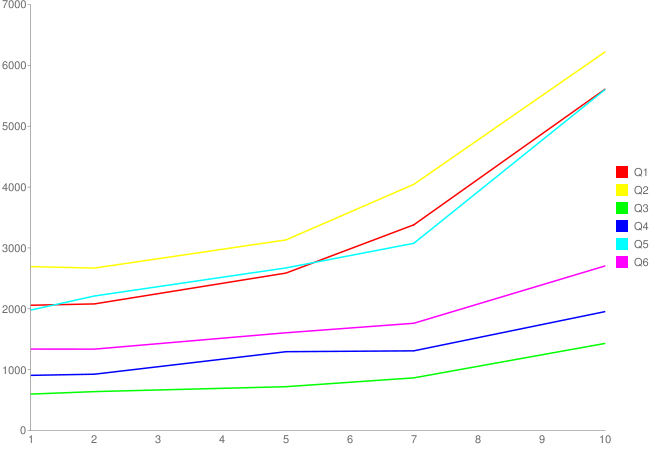
\includegraphics[width=0.85\textwidth]{figures/benchmark-4000.png}
	\caption{Durchschnittliche Response-Time bei einer Wartezeit von 4 Sekunden}
	\label{fig:benchmark-4000}
\end{figure}
 
 Man sieht dass die Berechnung von Q3 (Detailergebnisse Wahlkreis) am schnellsten ist, w�hrend die Berechnung von Q2 (Abgeordneten)
 am l�ngsten dauert.
 
 \newpage
 \subsection{Q1 - Q6 mit 2 Sekunden Wartezeit}
 
 Das Benchmark-Ergebnis mit einer reduzierten Wartezeit von jeweils \emph{zwei} Sekunden pro Browser zwischen den Queries:
 
 \begin{figure}[htbp]
	\centering
		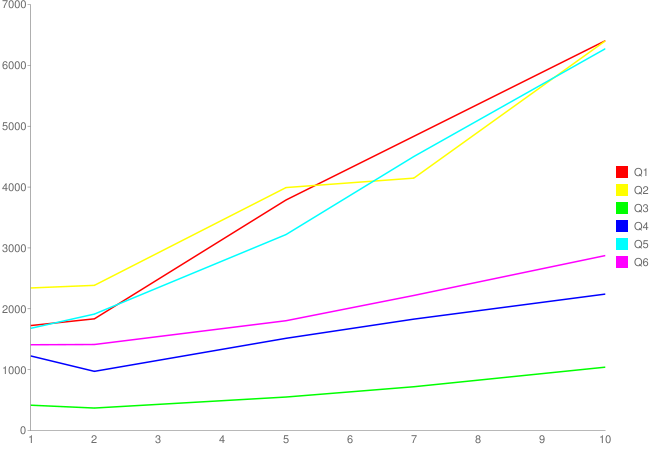
\includegraphics[width=0.85\textwidth]{figures/benchmark-2000.png}
	\caption{Durchschnittliche Response-Time bei einer Wartezeit von 2 Sekunden}
	\label{fig:benchmark-2000}
 \end{figure}
	
 Bei noch h�herer Server-Belastung ben�tigen die Queries Q1, Q2 und Q5 bei 10 parallelen Browsern schon durchschnittlich mehr als 7 Sekunden
 um zu antworten.
	
 \newpage
 \subsection{Q1 - Q6 mit 4 Sekunden Wartezeit und \texttt{WITH}-Tables}
 
 Das Benchmark-Ergebnis mit einer Wartezeit von vier Sekunden unter der Verwendung von \texttt{WITH}-Tables:
 
 \begin{figure}[htbp]
	\centering
		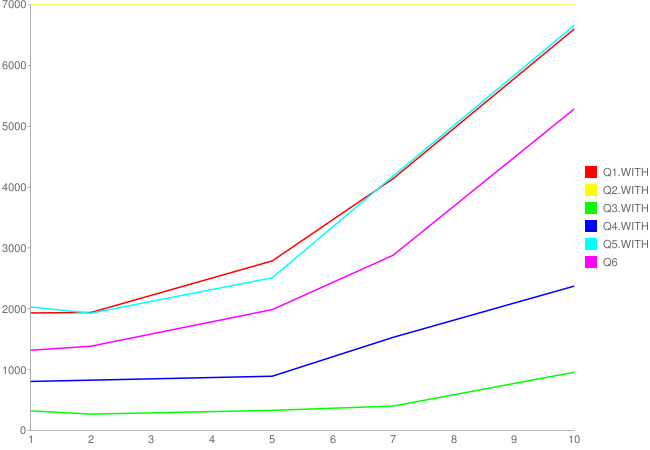
\includegraphics[width=0.85\textwidth]{figures/benchmark-WITH-4000.png}
	\caption{Durchschnittliche Response-Time bei einer Wartezeit von 4 Sekunden unter Verwendung von \texttt{WITH}-Tables}
 \end{figure}
 
 Man sieht sofort dass Q2 durch \texttt{WITH}-Tables deutlich langsamer geworden ist. Die anderen Queries sind dadurch
 im Allgemeinen etwas schneller geworden, insbesondere Q3.
 
 \newpage
 \subsection{Q1 - Q6 mit 2 Sekunden Wartezeit und \texttt{WITH}-Tables}
 
 Das Benchmark-Ergebnis mit einer Wartezeit von zwei Sekunden unter der Verwendung von \texttt{WITH}-Tables:
 
 \begin{figure}[htbp]
	\centering
		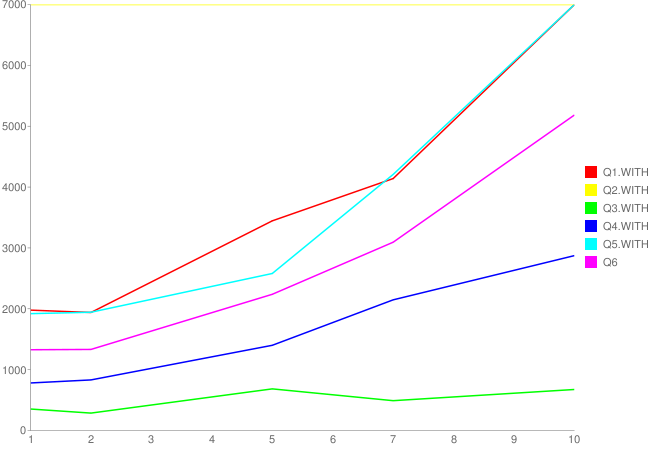
\includegraphics[width=0.85\textwidth]{figures/benchmark-WITH-2000.png}
	\caption{Durchschnittliche Response-Time bei einer Wartezeit von 2 Sekunden unter Verwendung von \texttt{WITH}-Tables}
 \end{figure}
 
 Bei noch h�herer Server-Belastung skalieren Q3 und Q5 mit \texttt{WITH}-Tables besser als ohne.
 
 \newpage
 \subsection{Q7 mit 2 Sekunden Wartezeit}
 
 Das Benchmark-Ergebnis von Q7 mit einer Wartezeit von zwei Sekunden einmal mit tempor�ren Tabellen und einmal mit \texttt{WITH}-Tables:
 
 \begin{figure}[htbp]
	\centering
		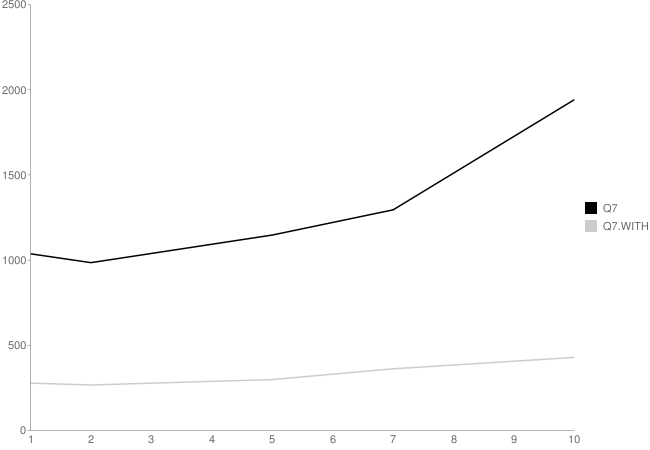
\includegraphics[width=0.85\textwidth]{figures/benchmark-Q7-2000.png}
	\caption{Durchschnittliche Response-Time bei einer Wartezeit von 2 Sekunden}
 \end{figure}

 Auch Q7 ist mit \texttt{WITH}-Tables performanter als ohne.
 
 \subsection{Interpretation der Ergebnisse}
Auf die Laufzeit der Queries wirken sich mehrere Faktoren aus. Wichtige Faktoren sind:
\begin{itemize}
	\item Effizienze Gestaltung der Queries (z.B. korrelierte Unterabfragen vermeiden)
	\item Optimierung des Anfragebaumes
	\item Leistungsf�higkeit der Hardware
	\item Caching von Ergebnissen durch das DBMS
	\item Vorhandensein von geeigneten Index-Strukturen
\end{itemize}

Bei der Durchf�hrung der Queries ist aufgefallen, dass die erste Anfrage oft um Gr��enordnungen l�nger f�r die Ausf�hrung braucht, als die folgenden Abfragen. Der Grund hierf�r ist, dass das DBMS Ergebnisse von zeitnah durchgef�hrten Anfragen oft Speichert um sp�tere Anfragen schneller durchf�hren zu k�nnen. Im Extremfall wird also das Endergebnis gespeichert und nicht neu berechnet. In der vorliegenden Arbeit w�rde also das DBMS am besten abschneiden, dass exakt die Ergebnistabellen der letzten Anfragen zwischenspeichert. Den st�rksten Effekt auf die Laufzeit haben Optimierungen, die das DBMS dazu bringen mehr von der Endergebnistabelle zu cachen. Dies ist im vorliegenden Benchmark wohl der Hauptgrund f�r Performanzunterschiede zwischen SQL-Abfragen basierend auf ``WITH''-Befehlen und SQL-Abfragen basierend auf Global Temporary Tables. Der Grund daf�r, dass die Anfragen unter Verwendung von ``WITH''-Befehlen teilweise auch deutlich langsamer sind, als die Anfragen mit temporary tables ist dementsprechend vermutlich ebenfalls auf andere Caching Eigenschaften zur�ckzuf�hren. In einer realen Implementierung sollte der Entwickler das Caching selber �bernehmen und bei jeder Browser Anfrage nur die minimal n�tigen Informationen neu berechnen.

Zus�tzlich hat die Verwendung von ``WITH'' Befehlen auch den Effekt, dass das DBMS die Anfrage besser optimieren kann, da alle Teiltabellen auf einmal zur Verf�gung stehen.




			
			\chapter{Stimmabgabe}
Die Stimmabgabe im Wahlinformationssystem l�uft wie folgt ab. Der W�hler erscheint im Wahllokal seines Wahlbezirkes. 
Dort legt er seinen Personalausweis vor. Durch die Vorlage des Personalausweises wird verhindert dass eine nicht-autorisierte
Person eine Stimme abgeben kann. Der Wahlhelfer vor Ort gibt die Personalausweisnummer in der vorgesehenen Weboberfl�che ein: 

\begin{figure}[htbp]
\centering
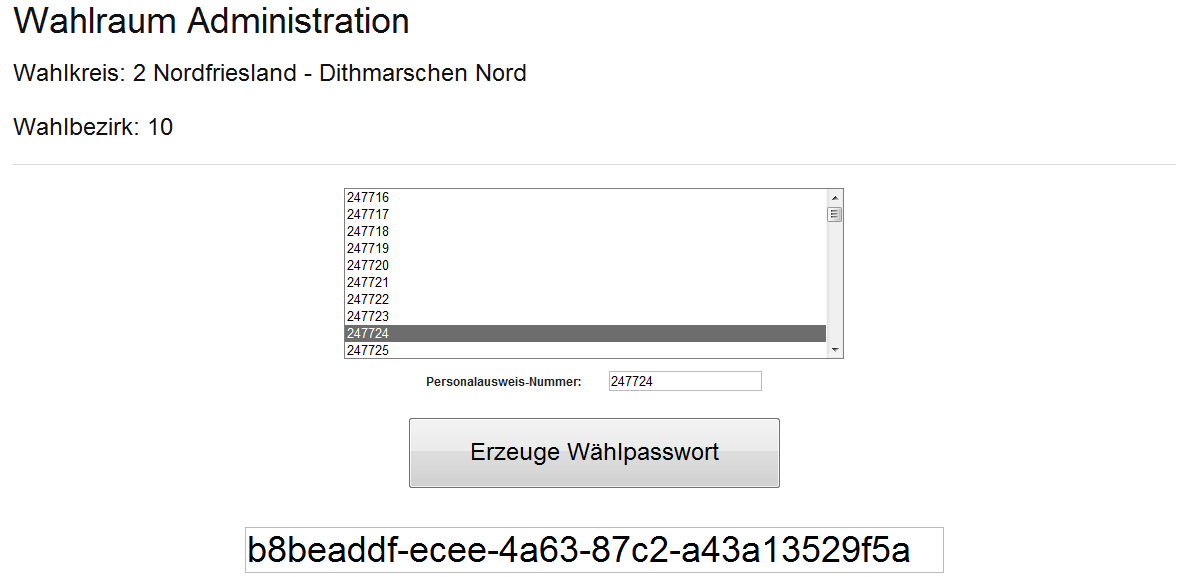
\includegraphics[width=0.6\textwidth]{figures/wahlraum-screenshot.png}
\caption{Webschnittstelle zur Eingabe der Personalausweis-Nummer}
\label{fig:wahlraum-screenshot}
\end{figure}

Das System pr�ft ob die Personalausweisnummer ein stimmberechtigter W�hler ist (Aus\-weis\-num\-mer ist berechtiger W�hler in Wahlkreis und Wahlbezirk). 
Wenn ja, wird gepr�ft ob dieser nicht bereits seine Stimme abgegeben hat (Flag \emph{gew�hlt} muss auf \emph{false} gesetzt sein). 
Hat er noch nicht gew�hlt, generiert das System ein zuf�lliges, zentral auf dem Server gespeichertes W�hlpasswort, das der Wahlhelfer dem 
W�hler beispielsweise auf einem Datentr�ger �bergibt. Durch die Generierung des W�hlpassworts wird das Flag \emph{gew�hlt} auf \emph{true} gesetzt. 
Dadurch wird verhindert dass der gleiche W�hler mehrfach w�hlen kann. 

\section{Wahlzettel}

Das W�hlpasswort berechtigt den W�hler an einem Wahlcomputer (der sich idealerweise im Wahlraum befindet) seine Stimme abzugeben:

\begin{figure}[htbp]
\centering
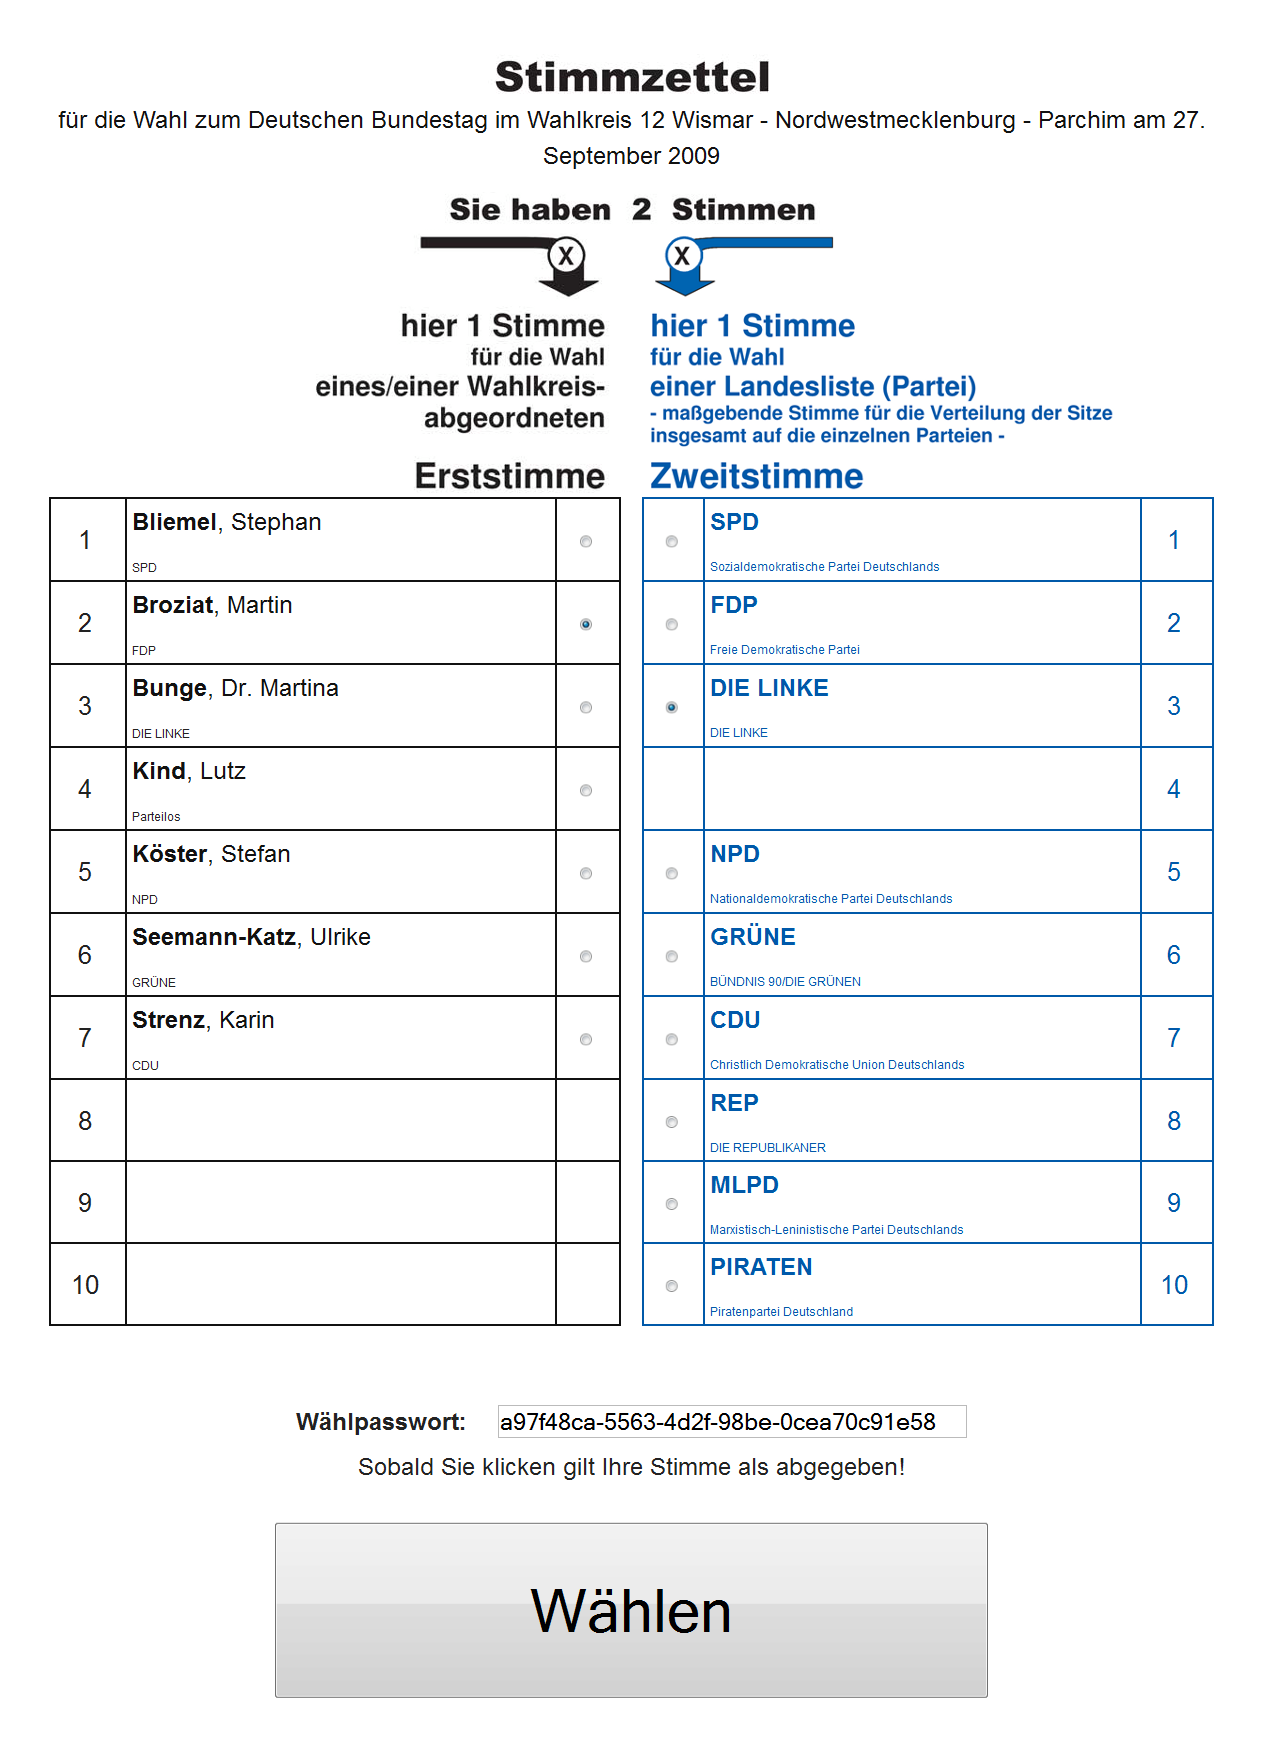
\includegraphics[width=0.85\textwidth]{figures/wahlzettel-screenshot.png}
\caption{Digitaler Wahlzettel mit W�hlpasswort}
\label{fig:wahlzettel-screenshot}
\end{figure}

Sobald der W�hler seine Kreuze gemacht hat, �berpr�ft das
System das eingegebene W�hlpasswort. Wenn es korrekt ist, wird die Stimme gez�hlt und das W�hlpasswort erlischt. 
Durch die Indirektion �ber das anonyme W�hlpasswort wird maximaler Datenschutz gew�hrleistet. 

Es gibt keinerlei Verbindung zwischen Personalausweisnummer und W�hlpasswort. Genauso wenig wie zwischen W�hlpasswort
und abgegebenen Stimmen. Das W�hlpasswort ist allerdings mit seinem Wahlkreis und Wahlbezirk verbunden. Dadurch wird der
Fall verhindert, dass der W�hler sein erhaltenes W�hlpasswort in einem anderen Wahllokal abgeben kann und so die 
Statistik verf�lscht.

Alle �bertragungen vom Wahllokal zum Server m�ssen gesichert sein. Da sichere Ver\-bin\-dung\-en nicht Thema dieses Projektes sind, 
wird in der Implementierung davon ausgangen, dass die Sicherung der Verbindung au�erhalb erfolgt.

\section{Auswertung}
Durch einen bestimmten Befehl im Webinterface kann die Ausz�hlung der Stimmen auf Wahlkreisebene angesto�en werden. Es wird davon ausgegangen, dass der Befehl nur dem Organisator bekannt ist und nur von physisch gesch�tzten Orten aus gegeben werden kann. In unserer Implementierung wird die Ausz�hlung durch \url{http://localhost:8080/WahlWebsite/ShowResult?query=refreshvotes} ausgel�st. Der Begriff refreshvotes steht dabei als Beispiel f�r einen m�glichen geheimen Befehl. Tats�chlich sollte dieser Befehl einem langen Passwort entsprechen. Die Ausz�hlung darf erst nach Schlie�\-ung des letzten Wahllokales ausgel�st werden. Die Sicherung der Auswertungsfunktion ist n�tig, um zu verhindern, dass st�ndig hochaktuelle Ergebnisse verf�gbar sind. Hochaktuelle Ergebnisse w�rden es in Einzelf�llen m�glich machen, auf die Stimmabgabe von Einzelpersonen zu schlie�en, indem das Ergebnis vor der Stimmabgabe mit dem Ergebnis nach der Stimmabgabe verglichen wird.
 
\end{document}

